% Intended LaTeX compiler: pdflatex
\documentclass[a5paper]{memoir}
\makeatletter

\usepackage{vocabulary}

\def\maketitle{}

\usepackage{eso-pic}

\newcommand*{\casesLegendHeaderBG}{%
  \AddToShipoutPictureBG{%
    \put(\LenToUnit{\paperwidth-25mm-\spinemargin},\LenToUnit{\paperheight-84mm}){%
      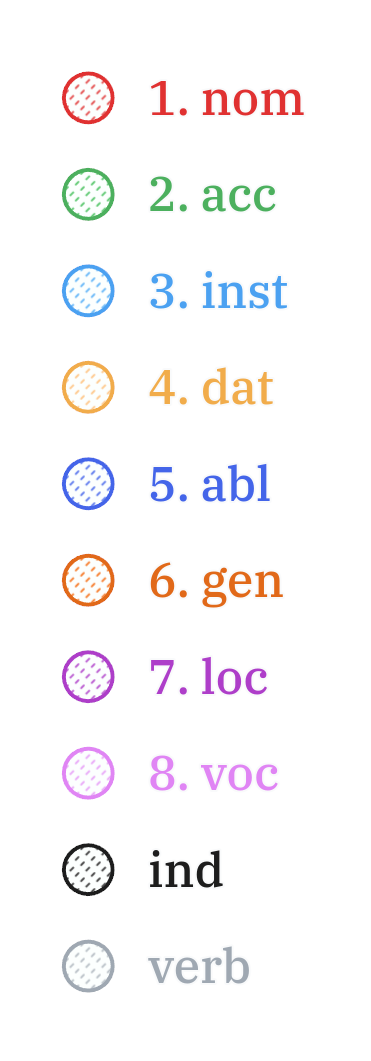
\includegraphics[width=25mm]{./images/cases-legend-white-large.png}%
    }%
  }%
}

\newcommand*{\casesLegendHeaderBGHere}{%
  \AddToShipoutPictureBG*{%
    \put(\LenToUnit{\paperwidth-25mm-\spinemargin},\LenToUnit{\paperheight-84mm}){%
      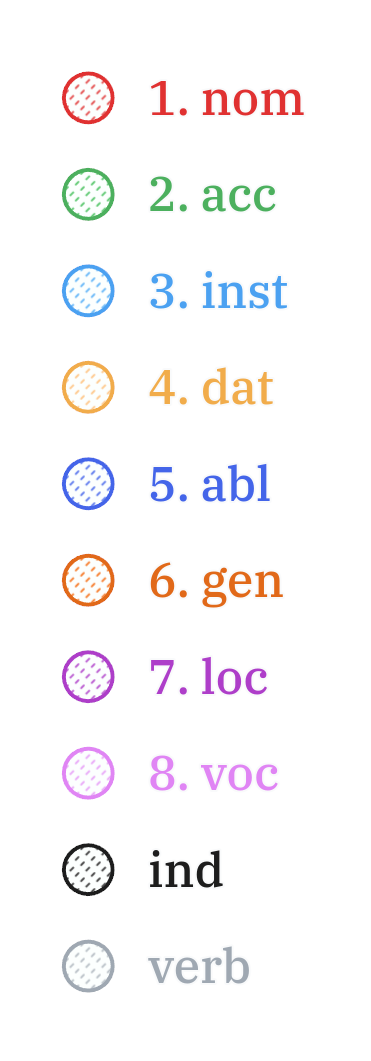
\includegraphics[width=25mm]{./images/cases-legend-white-large.png}%
    }%
  }%
}


\makeatother

\setcounter{secnumdepth}{2}
\date{\today}
\title{Vocabulary: Words}
\hypersetup{
 pdfauthor={The Bhikkhu Saṅgha},
 pdftitle={Vocabulary: Words},
 pdfkeywords={},
 pdfsubject={},
 pdfcreator={Emacs 30.1 (Org mode 9.7.11)}, 
 pdflang={English}}
\begin{document}

\chapter{Vocabulary: Words}
\label{sec:org2139963}

\begin{longtable}{L{0.48\linewidth} L{0.48\linewidth} H}
able to keep going; sustainable & yāpanīya (adj.) & \\
afflicted (with); victim (of); immersed (in) & otiṇṇa (pp. of otarati) & \\
after; beyond & paraṁ (ind.) & \\
after death; lit. going on & pecca (ind.) & \\
after & pacchā (ind.) & \\
afterwards; later; in the future & pacchā (ind.) & \\
again; once more & puna (ind.) & \\
agreeable; nice & piyarūpa (adj.) & \\
allows (to); permits (to) & anujānāti & \\
alms food; lit. lump dropping & piṇḍapāta (m.) & \\
alms food; lit. lump-like thing & piṇḍaka (m.) & \\
alteration (to); improvement (to) & vikappa (m.) & \\
always & sabbadā (ind.) & \\
a monk who; but whichever monk & yo pana bhikkhu (idiom) & \\
(1) analyses; dissects (2) divides; distributes; shares & vibhajati & \\
and what is more; and so too & puna caparaṁ (idiom) [puna + ca + paraṁ] & \\
and yet; however; still & api ca kho (idiom) & \\
another; other; different & añña (pron.) & \\
ant & kipillika (m.) & \\
appears; arises; takes place & uppajjati & \\
applies (attention); pays; lit. puts down & odahati & \\
approaches; goes to; visits & upasaṅkamati & \\
arising; appearing & uppāda (m., from uppajjati) & \\
arranges, organises, plans & saṁvidahati [saṁ + vi + √dhā + a + ti] & \\
arranging, organising, planning & saṁvidhāya (ger. of saṁvidahati) & \\
arrogantly; with an attitude; lit. having raised trunk high & uccāsoṇḍaṁ paggahetvā (idiom) & \\
as another; as alien & parato (ind.) & \\
ascetic; renunciant; holy man; monk; recluse; lit. who makes an effort; calm one & samaṇa (m.) [√sam + aṇa] & \\
asks; enquires; questions & pucchati & \\
assembly hall; meeting hall & upaṭṭhānasālā (f.) & \\
assembly; meeting; group & parisā (f.) & \\
assistance for the training & vinayānuggaha (m.) [vinaya + anuggaha] & \\
at some/any time & kudācanaṁ (ind.) & \\
attachment; taking as mine; sense of ownership & upadhi (m.) & \\
(1) attains; dwells in (2) engages in; performs & samāpajjati & \\
attains; enters on; becomes fully ordained & upasampajjati & \\
attendant; assistant & upaṭṭhāka (m.) & \\
attends & upaṭṭhāti & \\
attention; bringing-to-mind; observation; lit. making in mind & manasikāra (m.) [manasi + kāra] & \\
at the proper time & kālena (ind.) & \\
at the very most; for a maximum of & paramaṁ (ind.) & \\
avoids & vivajjati & \\
(1) ball; lump (2) bit of food & piṇḍa (m.) & \\
(1) banishes; drives away (2) makes ordain; ordains; lit. causes to leave & pabbājeti & \\
barks & bhussati & \\
barren; fruitless; sterile; unproductive & vañjha (adj.) & \\
bearable; tolearable & khamanīya (adj.) & \\
beautiful; lit. good colour & suvaṇṇa (adj.) & \\
becomes calm; ceases; is allayed & upasamati & \\
becomes detached (from); loses interest (in) & virajjati & \\
bed; sleeping place; couch; furniture & sayana (nt.) & \\
before; earlier & pure (ind.) & \\
before, previously & pubbe (ind.) & \\
before, previously & pubbe (ind.) & \\
beggar; mendicant & yācaka (m.) & \\
begins; starts; undertakes & ārabhati & \\
being; becoming; existence & bhava (m.) & \\
being; living being; lit. become & bhūta (nt.) [√bhū + ta] & \\
benefit (in); good result (of) & ānisaṁsa (m.) & \\
benefit; reason; purpose & atthavasa (nt.) & \\
best part; cream & maṇḍa (m.) & \\
beyond; across; over & pāraṁ (ind.) & \\
bird & sakuṇa (m.) & \\
blind person; lit. dark & andha (m.) & \\
blotched; stained & sabala (adj.) & \\
bodily behaviour; physical conduct & kāyasamācāra (m.) & \\
body; physical body & kāya (m.) & \\
body; physical body & kāya (m.) & \\
both & ubho (ind.) & \\
bowl; cup & mallaka (m.) & \\
boy & dāraka (m.) & \\
breaks; splits; shatters & bhindati & \\
brings & āharati & \\
broom & sammuñjanī (f.) & \\
brother & bhātar (m.) / bhātuka / bhāti & \\
brother(s); friend(s) & āvuso (ind.) [shortened from āyasmanto] & \\
burns; sets fire (to); burns down & ḍahati & \\
but nor do I & na panāhaṁ (idiom.) [na + pana + ahaṁ] & \\
but; rather; even & atha (ind.) & \\
but when; but because & yato ca kho (idiom) & \\
buys; purchases & kiṇāti & \\
by oneself for/to oneself & attanāva attano (idiom.) & \\
calamity; misfortune; lit. it comes & īti (f.) [√i + ti] & \\
calmed; tranquillised & samita (pp. of sammati) & \\
carefully reconsiders; re-inspects & anupekkhati & \\
carries; carries away; takes away & harati & \\
carrying; leading & vāha (adj.) & \\
carrying water (e.g. stream) & vārivaha (adj.) & \\
cat & biḷāra (m.) & \\
cattle; oxen & gāvo (m.) [go + āvo] & \\
causes an alteration; suggests an improvement & vikappaṁ āpajjati (idiom) & \\
certainly; definitely; lit. one point-ness & ekaṁsena (ind.) [eka + aṁsa + ena] & \\
change; alteration & vipariṇāma (m.) & \\
change; alteration & vipariṇāma (m.) & \\
changed, altered, distorted & vipariṇata (pp. of vipariṇamati) & \\
changes; alters; lit. completely bends around & vipariṇamati & \\
changes; alters; lit. completely bends around & vipariṇamati & \\
chews & khādati & \\
chief; headman; leader & gāmaṇi (m.) [gāma + aṇi] & \\
clean; clear; transparent & accha (adj.) & \\
clean; pure; bright; perfect & parisuddha (adj.) & \\
cleans; clears; purifies; lit. makes pure & sodheti & \\
closet; cupboard & koṭṭhaka (m.) & \\
cloth; clothes; robe & vattha (nt.) & \\
cloth; garments & dussa (nt.) & \\
coffee drink & kāphīpāna (nt.) & \\
cold & sīta (adj.) & \\
cold water & sītodaka (nt.) [sīta + udaka] & \\
comes & āgacchati & \\
comes back (to); falls back (on); lit. goes back & pacceti & \\
comfort; happiness; pleasure; contentment & sukha (nt.) & \\
coming; arrival & āgata (nt.) & \\
coming; arrival & āgata (nt.) & \\
community; monastic order & Saṅgha (m.) & \\
compassion; pity & anukampā (f.) & \\
(1) completely; fully (2) perfecly; rightly; correctly & sammā (ind.) & \\
completely comprehends; knows full well & parijānāti & \\
completely cooled; lit. blows away & nibbāti & \\
comprehends; understands & vijānāti & \\
concerning this life; regarding this world; relevant to here and now & diṭṭhadhammika (adj.) & \\
conduct; behaviour; activity & samācāra (m.) & \\
confesses & āvikaroti & \\
congee; sour gruel; rice husk porridge & kaṇājaka (nt.) & \\
considers as; takes as; regards as; lit. puts & dahati & \\
consumed; destroyed & khīṇa (pp. of khīyati) & \\
contact; sense impingement; touch & phassa (m.) & \\
continuity of the good teaching; longevity of the true doctrine & saddhammaṭṭhiti (f.) & \\
control; restraint; holding back & saṁvara (m.) & \\
controls; restrains & saṁvarati & \\
convinces; persuades; lit. causes to know & saññāpeti & \\
cook (noun) & sūda (m.) & \\
cooks (verb) & pacati & \\
Cool down / blow away the great passion! & Nibbāpehi mahārāgaṁ! & \\
could be; may be & siyā (opt.irreg. of atthi) & \\
country; province; area & janapada (m.) & \\
covers up; wraps over & onandhati & \\
cow; ox; cattle & go (m.) & \\
created, conditioned, fabricated; lit. put together & saṅkhata (pp. of saṅkharoti) [saṁ + √kar + ta] & \\
cries; weeps; wails & rodati & \\
cultivates; develops; lit. causes to become & bhāveti & \\
(1) danger; problem (2) disadvantage; drawback & ādīnava (m.) & \\
darkness; blackness; blindness; lit. blind making & andhakāra (m.) [andha + kāra] & \\
daughter & dhītar (f.) & \\
daughter of Māra & māradhītar (f.) & \\
day & aṇha (m.) & \\
day & diva (m.) / divasa (nt.) & \\
day-time & majjhanhikasamaya (m.) & \\
(1) death (2) schism; split; lit. breakup & bheda (m.) & \\
death; dying & maraṇa (nt.) & \\
death personified & māra (m.) & \\
defilement; impurity & kilesa (m.) & \\
delight; joy; rapture; feeling of love & pīti (f.) & \\
dependent; depending (on) & paṭicca (ger. of pacceti) & \\
descends (into); goes down (into) & otarati & \\
desires; longs (for) & nikāmeti & \\
desires; wants & icchati & \\
detached (from); without desire (for); lost interest (in) & viratta (pp. of virajjati) & \\
dies & mīyati & \\
diminishes; decreases; gets less; is lost & jīyati & \\
dirty; messy & uklāpa (adj.) & \\
disappears; vanishes; perishes; is destroyed & vinassati & \\
discharge; suppuration; outflow; effluent & āsava (m.) & \\
disciple; pupil; follower & sāvaka (m.) & \\
discipline; training; lit. leading out & vinaya (m.) & \\
discomfort; suffering; unease; stress & dukkha (nt.) & \\
discontent; aversion; boredom & aratī (f.) & \\
discontent; dislike & aratī (f.) & \\
discovered; found; attained; lit. arrived & adhigata (pp. of adhigacchati) & \\
discovery; finding; attainment; lit. arrival & adhigama (m.) & \\
disintegration; decay; old age; lit. going away & vaya (m.) [vi + √i + *a] & \\
does & karoti & \\
does not drown; does not overwhelm & nābhikīrati [na + abhi + √kir + a + ti] & \\
does not get to; does not obtain & nādhigacchati & \\
dog & sunakha (m.) & \\
Don't you do! & Mā akāsi! & \\
doubt; uncertainty & vicikicchā (f.) & \\
dries; desiccates; makes wither; lit. causes to dry up & visoseti & \\
drink; beverage & pāna (nt.) & \\
drinks; imbibes & pivati & \\
dropped; discarded; set aside & nikkhitta (pp. of nikkhipati) & \\
drowsiness; sluggishness & middha (nt.) & \\
dullness and drowsiness; sloth and torpor & thinamiddha (nt.) & \\
dullness; drowsiness; fuzziness; sluggishness & thina (nt.) & \\
dullness; sloth & thinamiddha (nt.) & \\
dwelling; building; house & agāra (nt.) & \\
ear hole; lit. ear stream & kaṇṇasota (nt.) & \\
ear & kaṇṇa (m.) & \\
ear & sota (nt.) & \\
earth; ground; floor & chamā (f.) & \\
ease; comfort; happiness; bliss & sukha (nt) & \\
easy; comfortable & phāsu (adj.) & \\
eaten; consumed & khādito (pp. of khādati) & \\
eats; enjoys & bhuñjati & \\
effort; energy & viriya (nt.) & \\
elder; senior monk & thera (m.) & \\
empty dwelling & suññāgāra (nt.) & \\
empty of; devoid of; without & suñña (adj.) & \\
enjoys; delights (in); takes pleasure (in) & abhiramati & \\
enjoys; finds pleasure (in) & ramati & \\
enters; goes into & pavisati & \\
enveloped (with); wrapped (with) & onaddha (pp. of onandhati) & \\
escape; exit; way out & nissaraṇa (nt.) & \\
eternal; ancient & sanantana (adj.) & \\
(1) ethical/moral conduct; virtue (2) behaviour; habit & sīla (nt.) & \\
evening-time & sāyanhasamaya (m.) & \\
ever; sometime & kadāci (ind.) & \\
excess; pleasure; indulgence & mada (m.) & \\
Excuse me! & Okāsa, bhante. & \\
exhausts, takes up in a excessive degree & pariyādāti & \\
(1) exists; is found; is present (2) is possible & vijjati [√vid + ya + ti] & \\
exists (in); is found (in); is present (in) & vijjati [√vid + ya + ti] & \\
expels (from); throws out; removes; lit. drags out & nikkaḍḍhati & \\
(1) experiences (2) produces (3) engages in (4) commits (an offense) (5) causes; effects & āpajjati & \\
externally; outside & bahi (ind.) & \\
face to face with & sammukha (adj.) & \\
fading of desire (for); dispassion (towards) & virāga (m.) & \\
(1) faith; belief (2) confidence (3) romantic devotion; lit. putting heart & saddhā (f.) & \\
(1) fall (2) drop; dropping; lit. made to drop & pāta (m.) & \\
falls & nipatati & \\
far side; far shore & pāra (nt.) & \\
fatigue; tiredness & kilamatha (m.) & \\
feeling & vedanā (f.) & \\
feels; experiences; senses; lit. causes to know & vedayati & \\
feels; experiences; senses & vedeti & \\
few; not much & appa (adj.) & \\
field of merit & puññakkhetta (nt.) & \\
field; plot of land & khetta (nt.) & \\
fifteen & pannarasa (card.) [pañca + dasa] & \\
fills up & paripūreti & \\
finds pleasure (in); is enamoured (with) & rajjati & \\
finds satisfaction (in) & vittiṁ āpajjati (idiom) & \\
fire & aggi (m.) & \\
first (1st); prime & paṭhama (ord.) & \\
flies up; files off; flies away & uḍḍayati & \\
focused on; lit. with such a mind & manasa (adj.) & \\
food; fuel; sustenance & āhāra (m.) & \\
food (lit. an enjoyable) & bhojanīya (m.) & \\
foot-washing water & pādodaka (m.) [pāda + udaka] & \\
for a long time & ciraṁ (ind.) & \\
for a week; for seven days & sattāhaṁ (ind.) & \\
forest; wood; wilds; wilderness & arañña (nt.) & \\
formerly, earlier & purā (ind.) & \\
form & rūpa (nt.) & \\
for those knowing; for those who understand & vijānataṁ (prp. of vijānāti) & \\
(1) for you; to you (2) your; yours & tuyhaṁ (pron.) & \\
fourteen & catuddasa / cuddasa (card.) & \\
friendliness; lit. non-hatred & avera (nt.) & \\
friend & mitta (m.) & \\
from far, from the further shore & pārato / parato (abl.) [para + to] & \\
from here & ito (ind.) & \\
from near, from the near shore & orato / apārato & \\
(1) from that (2) therefore; that is why & tasmā & \\
from there & tato (ind.) & \\
from travelling (from going on the journey) & addhānaṁ āgato & \\
(1) fruit; berry (2) consequence; result & phala (nt.) & \\
full (of); filled (with) & pūra (adj.) & \\
fully engaged; diligently practising & suppayutta (adj.) [su + payutta] & \\
fun; joke; play & dava (m.) & \\
gathers together; assembles; lit. falls together & sannipatati & \\
general (army) & senānī (m.) & \\
gets pleasure/pain; produces; engages in & āpajjati & \\
gets; receives; obtains & labhati & \\
gets; receives; obtains & labhati & \\
gets to; attains; obtains; lit. arrives at & adhigacchati & \\
gets up; gets out; arouses oneself; lit. stands up & uṭṭhahati; uṭṭhāti & \\
gift; donation & dakkhiṇā (f.) & \\
gives & deti & \\
gives up; abandons; lets go (of) & pajahati & \\
gives up; abandons & pajahati & \\
(1) giving; offering; generosity (2) alms; gift & dāna (nt.) & \\
giving up; abandoning & pahāya (ger. of pajahati) & \\
goal; purpose & attha (m.) & \\
goal; purpose; want & attha (m.) & \\
goes away, turns aside & apagacchati & \\
goes beyond; surpasses; transgresses & accayati & \\
goes forth (ordains as monk); lit. goes into exile & pabbajati & \\
goes & gacchati & \\
goes to; travels to & yāti & \\
gold & suvaṇṇa (nt.) & \\
gone to bed & sayanagata (adj.) & \\
good evening & susāyanha [su + sāya + anha] & \\
good midday & sumajjhanhika [su + majjha + anha + ika] & \\
Good morning (daybreak) Ven. Sir! & Suppabhātaṁ bhante. & \\
Good morning everyone. & Suppabhātaṁ sabbesaṁ. & \\
good morning & suppabhāta [su + pabhāta] & \\
goods; wares; merchandise & bhaṇḍa (nt.) & \\
grabs hold (of); seizes; takes & gaṇhāti & \\
granary; treasury; storehouse & koṭṭhāgāra (nt.) & \\
greeted & sammodi (aor. of sammodati) & \\
greets & sammodati & \\
growth; increase & virūḷhi (f.) & \\
growth (of); increase (of); lit. more state & bhiyyobhāva (m.) [bhiyyo + bhāva] & \\
guest & āgata (m.) & \\
guru; esteemed person & garu (m.) & \\
hall; shed & sālā (f.) & \\
hand; palm & pāṇi (m.) & \\
happiness (for); appreciation & muditā (f.) [√mud + ita + ā] & \\
harnesses; employs; applies & payuñjati & \\
has fun; amuses oneself (with) & saṅkelāyati (from kīḷati) & \\
hatred; hostility & vera (nt.) & \\
hatred; ill-will; animosity; hostility & vera (nt.) & \\
have reached; have arrived (at) & patta (pp. of pāpuṇāti) & \\
having abandoned the five hindrances & pañca nīvaraṇe pahāya (idiom) & \\
having eaten & bhutvā (abs. of bhuñjati) & \\
having got; having obtained & laddhā (abs. of labhati) & \\
having known & ñatvā / jānitvā & \\
having raised / held up & paggahetvā (ger. of paggaṇhāti) & \\
having taken; having grabbed hold (of) & gahetvā (abs. of gaṇhāti) & \\
having taken over the mind, it remains & cittaṁ pariyādāya tiṭṭhati (idiom) & \\
healthy; beneficial; good; wholesome & kusala (adj.) & \\
healthy; well; lit. able & kallaka (adj.) & \\
hearing from another person; word of another & parato ca ghoso (idiom) & \\
hears & suṇāti & \\
he attends to me & so maṃ upaṭṭhāti & \\
heavenly being; a god & deva (m.) & \\
he is (√as) & atthi & \\
he is (√hū) & hoti & \\
helpful; useful & upakāra (adj.) & \\
here & idha (ind.) & \\
here; in this place & atra (ind.) & \\
(1) here; now; in this world; (2) in this case & idha (ind.) & \\
he & so, sa (m.) & \\
he who attends to the ill & yo gilānaṃ upaṭṭhāti & \\
he who (m.nom.) & yo (m.) & \\
he who; whoever; whatever; whichever & yo (pron., masc.nom.sg. of ya) & \\
he will do; he will make & kāhati (fut.) [√kar + o + ti] & \\
highest; supreme & agga (adj.) & \\
highest; unsurpassed; incomparable; lit. nothing higher & anuttara (adj.) & \\
his & assa (pron.) & \\
hits; beats; stabs & hanati & \\
holding back; restraining; lit. holding down & niggaha (adj.) [ni + √gah + a] & \\
holds up; carries; bears in mind & dhāreti & \\
holds up; raises up & paggaṇhāti & \\
hole; crack & chidda (nt.) & \\
horse & assa (m.) & \\
hot & uṇha (adj.) & \\
hot water & uṇhodaka (nt.) [uṇha + udaka] & \\
house builder; mason; carpenter & gahakāra (m.) & \\
house; dwelling & geha (nt.) & \\
house; dwelling & geha (nt.) [√gah + a] & \\
householder; landowner & gahapatika (m.) [gaha + pati + ka] & \\
house; home; lit. entering down & nivesana (nt.) & \\
How indeed? Why on earth? & kiṁ nu kho (idiom) & \\
How? & kathaṁ (ind.) & \\
How? & kinti (ind.) & \\
how many? & kittaka (adj.) & \\
how many? & kittaka (adj.) [ka + tta + ka] & \\
how-old? lit. having how many years? & kativassa (adj.) & \\
human being; man; person & manussa (m.) & \\
I am (√as) & asmi & \\
I am (√hū) & homi & \\
I don't know. & Na jānāmi. & \\
I don't understand. & Na pajānāmi. & \\
(I feel) sorry. (for your situation) & Kāruññaṁ. & \\
if more than that & tato ce uttari (idiom) & \\
if not & no ce & \\
if & sace (ind.) & \\
if; whether; perhaps & yadi (ind.) & \\
I have (in my presence there are) & mama santike santi (idiom) & \\
I have (my things are) & mayhaṁ \ldots{} santi & \\
I hope; I trust & kacci (ind.) & \\
I hope you are\ldots{} & kacci'si [kacci + asi] & \\
illness; affliction & ābādha (m.) & \\
ill will; lit. going wrong & byāpāda (m.) & \\
immediately after that; with no interval & anantaraṁ (ind.) & \\
imposes (on); inflicts (on) & paṇeti & \\
in both cases; on both sides; lit. both matters & ubhayattha (ind.) [ubhaya + attha] & \\
indignant; angry; annoyed & kupita (pp. of kuppati) & \\
inflicts punishment; imposes a fine & daṇḍaṁ paṇeti (idiom) & \\
informs & āroceti & \\
in future & āyatiṁ (ind.) & \\
inspiration; faith; trust; confidence; lit. settling & pasāda (m.) & \\
intent; engaged & payutta (pp. of payuñjati) & \\
intention; volition; choice; lit. making together & saṅkhāra (m.) & \\
in the future; hereafter & samparāyika (adj.) & \\
in the presence (of); near (to) & santike (ind.) & \\
in those; among those & tesu (pron.) [ta + esu] & \\
in us; among us & amhesu (pron.) (1st.loc.pl of ahaṁ) & \\
in whatever way & yathā yathā (idiom) & \\
I (pron.) & ahaṁ & \\
irritated; annoyed; displeased; lit. not own mind & anattamana (adj.) [na + atta + mana] & \\
is abandoned; is given up & pahīyati (pr.pass. of pajahati) & \\
is able (to) & sakkoti & \\
is angered; is provoked; is irritated & kuppati & \\
is; being; becomes & bhavati & \\
(is) born & jāyati & \\
is burned; is scorched; is on fire & ḍayhati & \\
is calmed; is appeased & sammati & \\
is calmed; is appeased & sammati (pr. pass.) [samma + ti] & \\
is destroyed; is exhausted & khīyati & \\
is happy; enjoys himself; rejoices & modati [√mud + *a + ti] & \\
is happy (with); delights (in); likes; enjoys & nandati & \\
is hurt; is killed; is slaughtered & haññati (pr. pass. of hanati) & \\
is in solitude; seeks privacy & rahāyati & \\
is received; is obtained & labbhati (pass. of labhati) & \\
is said to be; is called & vuccati (pass. of vacati) & \\
is suitable; worthy (for); enough (for) & alaṁ (ind.) & \\
It is cold today. & Ajj'ātisītaṁ. & \\
It is hot today. & Ajj'āccuṇhaṃ. [ajja (ind.) + ati  + uṇha] & \\
it is possible, it is plausible; lit. a basis exists & ṭhānaṁ vijjati (idiom) & \\
it is suitable; it is allowable & kappati & \\
its; of/for that & tassa (gen./dat. of \emph{ta} 'it, that') & \\
it & taṁ, tad (nt.) & \\
it; that & ta / taṁ (pron.) & \\
jewel; gemstone & maṇi (m.) & \\
joy; happiness; pleasure; lit. gain & vitti (f.) & \\
just indeed; only just & h'eva (ind.) [hi + eva] & \\
Kaṭhina-cloth & kaṭhinadussa (nt.) & \\
king; ruler & rāja (m.) & \\
knower of the world (epithet of the Buddha) & lokavidū (m.) & \\
knows clearly; understands; distinguishes & pajānāti & \\
knows for oneself; personally realizes & sacchikaroti & \\
knows & jānati & \\
knows; understands & jānāti & \\
lamp; light; lighting & padīpa (m.) & \\
laughs; jokes & sañjagghati & \\
layman; male lay follower & upāsaka (m.) & \\
laywoman; female lay follower & upāsikā (f.) & \\
laziness; tiredness & tandī (f.) & \\
leads; carries away; takes away & neti & \\
leads (to); results (in); causes & saṁvattati & \\
learned by heart; mastered & pariyatta (adj. pp. of pariyāpuṇāti) & \\
length of life; life-span & āyuppamāṇa (nt.) [āyu + pamāṇa] & \\
lies down; rests; sleeps & sayati & \\
lies; lies around; lit. sleeps & seti & \\
light; brightness; clarity & āloka (m.) & \\
like; as; according to; how & yathā (ind.) & \\
like; as; according to; how & yathā (ind.) & \\
lion & sīha (m.) & \\
little fatigue; little tiredness & appakilamatha (m.) & \\
little; tiny; minute & thoka (adj.) & \\
lives (in); dwells & viharati & \\
lives & jīvati & \\
long road; journey & addhāna (nt.) & \\
long road; journey & addhāna (nt.) & \\
looking (at); observing; watching & anupassī (adj.) & \\
loves; holds dear; is fond of & piyāyati & \\
(1) man; person (2) servant; labourer (3) grammatical person & purisa (m.) & \\
man; person & nara (m.) & \\
many; much; a lot (of); great; large & bahu (adj.) [√bah + u] & \\
many people; many things; a lot & bahū (m.pl. of bahu) & \\
market; bazaar; market place & antarāpaṇa (m.) & \\
master; gentleman & ayya (m.) & \\
master; gentleman; sir & ayya (m.) & \\
meditates (on); contemplates; reflects (on) & upanijjhāyati & \\
meditative calm; lit. meditating & jhāna (nt.) & \\
mentally examines & manasānupekkhati & \\
merchant; trader; dealer & vāṇija (m.) & \\
merit; good deed & puñña (nt.) & \\
mind; heart; mental act & citta (nt.) & \\
monkey; ape & makkaṭa (m.) & \\
monk; mendicant; lit. beggar & bhikkhu (m.) & \\
moon & canda (m.) & \\
more; greater; bigger & bahutara & \\
more; greater; superior & bhiyyo (ind.) & \\
moreover; and so; but; or; however & pana (ind.) & \\
morning-time & pubbaṇhasamaya (m.) & \\
mother and father; parents & mātāpitar (m.) & \\
moved over; shifted; transferred & saṅkanta (pp. of saṅkamati) & \\
moved over, shifted, transferred & saṅkanta (pp. of saṅkamati) [saṁ + √kam + ta] & \\
moves about; wanders about & vicarati & \\
myself slept well & sukhamasayitthaṁ (aor.1st.refl.) & \\
my; to me; for me & me / mayha / mama (pron.) & \\
near side; near shore & ora (nt.) / apāra (nt.) & \\
neglects; omits & riñcati & \\
Never mind (leave it aside). & Tiṭṭhatu, bhante. & \\
never & na kadāci (idiom) & \\
new; fresh & nava (adj.) & \\
next; after & para (adj.) & \\
night & sāya (nt.) & \\
nods off; dozes off & pacalāyati & \\
No. & No hetaṁ, bhante. & \\
not I & nāhaṁ [na + ahaṁ] & \\
now & idāni (ind.) & \\
now, if a monk\ldots{}; further, \ldots{} & bhikkhu pan'eva (idiom) [pana + eva] & \\
(object of) pleasure; sensual pleasure & kāma (m.) & \\
object of sensual pleasure; lit. sensual strings & kāmaguṇa (m.) & \\
obligation; duty & kicca (nt.) & \\
observance day & uposatha (m.) & \\
observing the body; who watches the body & kāyānupassī (adj.) [kāya + anupassī] & \\
obstacle; obstruction; hindrance; lit. blocking & nīvaraṇa (m.) & \\
occurs; happens; befalls; lit. goes down & okkamati & \\
ocean & sāgara (m.) & \\
ochre robe & kāsāva (nt.) & \\
(of a tree) root; base (2) source; origin; root (3) money; cash & mūla (nt.) & \\
offence; transgression & āpatti (f.) & \\
offense; transgression & āpatti (f.) & \\
(of fire) extinguishing; quenching; going out; lit. blowing away & nibbāna (nt.) [nī + √vā + ana] & \\
(of fire) grows cold; lit. causes to blow away & nibbāpeti (caus. of nibbāti) & \\
of the best quality; lit. to be drunk like cream & maṇḍapeyya (adj.) & \\
(of the body) limb & gatta (nt.) & \\
of the teacher; master's; Buddha's & satthu (m.) [√sās + tar + u] & \\
(of time) passes; spends; wastes & atināmeti & \\
old age; growing old; decay & jara (m.) [√jar + a] & \\
one day & ekadā (ind.) & \\
one hundred & sata (card.) & \\
one slept well; one rested comfortably & sukhamasayittha (aor.2nd.pl.) & \\
one without faith or confidence & appasanna (m.) & \\
only; just; merely & eva (ind.) & \\
only; just; merely; exclusively & yeva & \\
organises; arranges; prepares (food; drinks; etc.) & paṭiyādeti & \\
our; of us; my (royal plural) & amhākaṁ (pron.) & \\
out of compassion; lit. taking pity & anukampaṁ upādāya (idiom) & \\
over; on; around (prefix) & anu- & \\
passes over to, shifts, transmigrates & saṅkamati & \\
passes over to, shifts, transmigrates & saṅkamati & \\
passion; infatuation; lust & rāga (m.) & \\
paying proper attention; wise reflection; lit. attention to the source & yoniso manasikāra (idiom) & \\
pedestrian, traveller & pathika (m.) & \\
personal; lit. see for oneself & sacchi (adj.) & \\
personal; lit. see for oneself & sacchi (adj.) & \\
personal; lit. see for oneself & sacchi (adj.) & \\
personally experiences, realizes; lit. personally does & sacchikaroti & \\
personally; with one’s own hand & sahatthā (ind.) & \\
person; individual & puggala (m.) & \\
(1) picks up (2) takes; accepts (3) grasps; learns & uggaṇhāti & \\
(1) piece; part (2) broken; defective (3) chip; break; failure & khaṇḍa (m.) & \\
(1) place (2) reason; ground; basis;  lit. standing & ṭhāna (nt.) & \\
(1) place; region (2) point; item; detail & desa (m.) & \\
places down; lays down; sets up & odahati & \\
playing together & saṅkīḷati [saṁ + √kīḷ] & \\
plays (with); has fun (with) & kīḷati & \\
Please sit. & Nisīdatha. & \\
pleasure; enjoyment; relish; delight & nandi (f.) & \\
plows; tills; turns the soil & kasati & \\
ponders; reflects; thinks about & anuvitakketi & \\
Portugal-region & Portugal-desa & \\
practices; engages in; lit. yokes near & anuyuñjati & \\
practices; engages (in) & paṭisevati & \\
preference; approval & ruci (f.) & \\
prepares; arranges; considers & kappeti & \\
prepares; sets out (a seat, etc.) & paññāpeti & \\
previous; old; ancient & purāṇa (adj.) & \\
prince & rājakumāra (m.) & \\
privacy; solitude; lit. sticking to oneself & paṭisallāna (nt.) & \\
privately; alone; secretly & raho (ind.) & \\
produces; comes up with & abhinipphādeti & \\
properly; prudently; thoroughly; lit. to the source & yoniso (ind.) [yoni + so] & \\
protects; guards & rakkhati & \\
pulls (towards); tugs (to) & āviñchati & \\
punishment; fine & daṇḍa (m.) & \\
purity; purification & pārisuddhi (f.) & \\
(1) puts together; composes; fabricates (2) restores & saṅkharoti & \\
rain; downpour & vassa (m.) & \\
rains & vassati & \\
reaches; arrives (at) & pāpuṇāti & \\
realizing; achieving; attaining; lit. doing personally & sacchikaraṇa (nt.) & \\
really enjoying; very fond (of) & abhirata (adj. pp. of abhiramati) & \\
recently, soon & aciraṁ (ind.) & \\
recites & uddisati & \\
relishes; takes pleasure (in) & assādeti & \\
remorse; regret; lit. remembering back negatively & vippaṭisāra (m.) & \\
repeatedly; again and again & punappunaṁ (ind.) & \\
requisite; everyday item & parikkhāra (m.) & \\
restlessness; agitation & uddhaccakukkucca (nt.) & \\
resulting in; producing; lit. coming up & udraya (adj.) & \\
returns; steps back; goes away; lit. goes back & paṭikkamati & \\
reverence (to); homage (to); lit. bow & namas (m.) [√nam + as] & \\
rice & bhatta (m.) & \\
rice; boiled rice; food; lit. wet stuff; boiled in water & odana (m.) & \\
rice gruel; congee & yāgu (f.) & \\
rice gruel; rice water & acchakañjiyā (f.) & \\
(1) rice water; congee (2) glue; sticky stuff & kañjiya (nt.) & \\
right here & ettheva [ettha + eva] & \\
right view; correct outlook & sammādiṭṭhi (f.) & \\
rising (from); emerging (from) & uṭṭhāya (ger. of uṭṭhahati) & \\
root (of a tree); base; foot & mūla (nt.) & \\
runs & dhāvati & \\
sage; hermit & muni (m.) & \\
sage; wise man & paṇḍita (m.) & \\
(1) sal tree (2) brother-in-law & sāla (m.) & \\
says; speaks & vadeti & \\
scatters over; sprinkles & abhikīrati & \\
scribe, clerk, writer & lekhaka (m.) & \\
seat; chair; lit. sitting & āsana (nt.) & \\
seclusion; discrimination & viveka (m.) & \\
seclusion; solitude & viveka (m.) & \\
seed; germ & bīja (nt.) & \\
seen; found; visible & diṭṭha (pp. of √dis) & \\
sees; observes; watches & anupassati & \\
sees & passati & \\
sees; takes a look (at) & pekkhati & \\
sees; takes a look (at) & pekkhati & \\
(See you) tomorrow. & Suve. & \\
sells & vikkiṇāti & \\
servant; attendant & sevaka (m.) & \\
sets out; provides; lit. causes to stand near & upaṭṭhāpeti [upa + √ṭhā + *āpe + ti] & \\
she (f.) & sā (f.) & \\
She speaks to him/them. & Sā taṃ bhāsati. & \\
shines; blazes; burns & tapati & \\
shines (in); looks beautiful (in) & sobhati & \\
should be shared with & saddhiṁ saṁvibhajitabbaṁ & \\
sick; ill; unwell & gilāna (adj.) & \\
silence, quiet & tuṇhī (ind.) & \\
silver coin; money; cash & rūpiya (nt.) & \\
sister & bhaginī (f.) & \\
sits & nisīdati & \\
sitting alone & ekamāsīna (adj.) [eka + āsīna] & \\
sitting hall & āsanasālā (f.) & \\
sitting place; seat & nisajjā (f.) & \\
skin & taca (m.) & \\
sky & ākāsa (m.) & \\
sleeps well (happily); rests comfortably & sukhaṁ seti (idiom) & \\
slept well; rested comfortably & sukhamasayi (aor.2nd/3rd.sg.) & \\
some or other; even some; just some & kocideva & \\
soot; ash & masi (m.) & \\
sorrows; grieves; mourns & socati & \\
(Sorry, I have) regret. & Vippaṭisāraṁ. & \\
(Sorry,) I'll make amends. & Paṭikarissāmi. & \\
(1) sound; voice; utterance (2) rumour; report (3) cry; shout & ghosa (m.) & \\
soup; broth & yūsa (m.) & \\
(1) sows; plants (2) shaves & vapati & \\
speaks & bhāsati & \\
speaks & vacati & \\
speech; talk & bhāsa (m.) & \\
spoon & kaṭacchu (m.) & \\
spotted; blemished & kammāsa (adj.) & \\
stability; continuity; longevity; lit. standing & ṭhiti (f.) & \\
stands & tiṭṭhati & \\
state; condition; nature & bhāva (m.) & \\
stays; dwells & vasati & \\
steals; robs & coreti & \\
stream; river & sota (m.) & \\
string; thread; tie & guṇa (m.) & \\
striving (in); active (in); lit. going out & nikkāmī (adj.) [nī + √kam + *ī] & \\
strokes; massages; rubs; lit. wipes along & anumajjati [anu + √majj + a + ti] & \\
strong; firm; steady & daḷha (adj.) & \\
studies well; learns thoroughly; masters; lit. reaches & pariyāpuṇāti & \\
suitable time (for) & pattakalla (nt.) & \\
sun; lit. shining & suriya (m.) & \\
sunrise; dawn; daybreak & pabhāta (nt.) & \\
support; help; assistance & anuggaha (m.) [anu + √gah + a] & \\
(1) support; requisite; necessity (2) cause; reason; condition (for) & paccaya (m.) & \\
sweeping & sammajjana (nt. from sammajjati) & \\
sweeping that place & taṇṭhāna-sammajjanaṁ & \\
sweeps; cleans & sammajjati [saṁ + √majj + a + ti] & \\
takes; accepts; receives & paṭiggaṇhāti & \\
takes; accepts; receives & paṭiggaṇhāti & \\
takes a seat; sits down; lit. prepares a seat & nisajjaṁ kappeti (idiom.) & \\
(1) takes; grasps; embraces (2) steals; takes (3) obeys; follows; accepts; lit. takes & ādiyati & \\
takes; grasps (onto); lit. takes near & upādiyati & \\
takes & harati & \\
(1) taking; grasping; embracing (2) receiving; accepting & ādāya (ger. of ādiyati) & \\
taking; grasping (onto); lit. taking near & upādāya (ger. of upādiyati) & \\
talks; speaks; converses & sallapati & \\
teacher; master & satthar (m.) [√sās + tar] & \\
teacher; religious leader & ācariya (m.) & \\
teaches; explains & deseti & \\
ten & dasa (card.) & \\
Thank you. & Anumodāmi. & \\
that much; that far; still; at least & tāva (ind.) & \\
the born & jāta (pp. of jāyati) & \\
theft; stealing; lit. taking what is not given & adinnādāna (nt.) & \\
(1) then; after that (2) yet; but still; however & atha kho (idiom.) & \\
therefore; in that case; if that's so & tena hi & \\
there; in that place & tahiṁ (ind.) & \\
there & tattha / tatra (ind.) & \\
the reverence (to); the homage (to); lit. bow & namo (ind.; nom.sg. of namas) & \\
these & ime / imā / imāni (pron.) & \\
they are (√as) & santi & \\
they are (√hū) & honti & \\
they (f.) & tā, tāyo (f.) & \\
they go to; they travel to & yanti (3rd.pl of yāti) & \\
they (m.) & te (m.) & \\
they (nt.) & tāni (nt.) & \\
thief; robber & cora (m.) & \\
(1) thinks (about) (2) meditates; contemplates (3) broods (4) burns & jhāyati & \\
thinks; presumes; supposes & maññati & \\
this; he; it & esa (pron.) & \\
this; he; it & esa (pron.) & \\
this indeed; certainly this & hidaṁ (sandhi.) [hi + idaṁ] & \\
this is his & ayamassa & \\
this is mine & meso & \\
this; this person; this thing & ayaṁ (pron.) & \\
this; this person; this thing & ayaṁ (pron.) & \\
thought; reflection & vitakka (m.) & \\
(1) throws down; discards (2) puts down (3) keeps; stores & nikkhipati & \\
throws down; discards; drops & nikkhipati & \\
time; occasion & samaya (m.) & \\
to ask; to question (infinitive) & pucchituṁ & \\
to buy & ketuṁ / kiṇituṁ & \\
to converse (with) & sallapituṁ (inf. of sallapati) & \\
today & ajja (ind.) & \\
to do; to make & kātuṁ (inf.) & \\
to/for her; to/for that & tassā (f.dat.sg.pron.) [ta + ssā] & \\
to/for the cow, the cow's (irregular form) & gavassa, gāvassa & \\
together with / accompanied by & saddhiṁ, saha (ind.) & \\
to lie down; to sleep & sayituṁ & \\
(1) to me; for me (2) my; mine & mayhaṁ (pron.) & \\
to me & maṁ & \\
too hot & accuṇha (adj.) [ati + uṇha] & \\
tooth-stick; toothbrush & dantapona (nt.) & \\
to see (infinitive) & passituṁ & \\
to sell & vikkiṇituṁ (inf. of vikkiṇāti) & \\
to stay (infinitive) & vasituṁ & \\
touched (by); contacted (by) & phuṭṭha (pp. of phusati) & \\
touches; contacts; feels & phusati & \\
to where? & kuhiṁ (ind.) [ka + hiṁ] & \\
(1) town; city (2) fortress; stronghold & nagara (nt.) & \\
town; market town & nigama (m.) & \\
(1) to you; for you (2) your; of you & tava (pron.) & \\
to you; for you & tava (pron.) & \\
tree & rukkha (m.) & \\
trouble; misfortune; pain; misery & agha (nt.) & \\
trunk of pride; raised trunk (of an elephant) & uccāsoṇḍā (f.) [uccā + soṇḍā] & \\
truth & sacca (nt.) & \\
twenty & vīsati (card.) [dvi + dasa + ti] & \\
unbeneficial; harmful & ahitāya (dat.sg. of na + hita) & \\
undertaking; entering on; attaining & upasampajja (ger. of upasampajjati) & \\
unrepentant; obdurate; obstinate; lit. difficult to embarrass into silence & dummaṅku (adj.) [dur + maṅku] & \\
untreated soup; bean broth & akaṭayūsa (m.) & \\
untroubled; carefree; problem-free & anagha (adj.) [na + agha] & \\
venerable; reverend & āyasmant (m.) & \\
view; belief; opinion & diṭṭhi (f.) & \\
village; hamlet & gāma (m.) & \\
Wait (stay) here. / May you wait here. & Ettheva tiṭṭha / tiṭṭhatha. & \\
walking tour; walking journey & cārikā (f.) & \\
walks & carati & \\
wanders on tour; walks about & cārikaṁ carati (idiom.) & \\
wanting; lit. over thinking & abhijjhā (f.) & \\
warding off; repelling; driving off & paṭighāta (m.) & \\
washes; cleans; rinses & dhovati & \\
washing water; rinsing water; lit. to be used & paribhojanīya (adj.) & \\
was lost & jīyittha (aor. 3rd. refl. sg. of jīyati) & \\
water; drinking water; lit. to be drunk & pāṇīya (nt.) & \\
water (stream) & vāri (nt.) & \\
water & udaka (nt.) & \\
we are (√as) & asma & \\
we are (√hū) & homa & \\
(1) wearing away; exhausting (2) obsessing; overpowering; lit. completely seizing & pariyādāya & \\
wearing away; destruction & khaya (m. from khīyati) & \\
we could be; we may be (√as) & assāma (opt. pl. of assa) & \\
Welcome here. & Svāgataṁ. & \\
welfare (of); benefit (of); blessing & hita (nt.) & \\
well-behaved; good; honest & pesala (adj.) & \\
well-being; excellence & suṭṭhutā (f.) & \\
well-being; prosperity & suvatthi (f.) [su + √as + ti] & \\
well; good; right & suṭṭhu (ind.) & \\
we & mayaṁ & \\
When? & kadā (ind.) & \\
when \ldots{} then \ldots{} & yadā \ldots{} tadā \ldots{} (idiom) & \\
when; whenever & yadā (ind.) & \\
where? from where? & kuto (ind.) & \\
where?; from where? & kuto (ind.) [ka + to] & \\
Where is the market? & Kattha antarāpaṇo? & \\
Where? & kattha (ind.) & \\
white & seta (adj.) & \\
who has faith (in); who has confidence (in); lit. settled & pasanna (adj.) & \\
who has made merit; has gained spiritual wealth & katapuñña (adj.) [kata + puñña] & \\
whose; of/for whom & yassa (gen./dat. of ya 'who') & \\
who?; what?; which? & ka / ko (pron.) & \\
Why is that? Of what cause? & Taṁ kissa hetu? & \\
why?; lit. from what? & kasmā (ind.) [ka + smā] & \\
will bring & āharissati & \\
wise man; knowledgable man & viññū (m.) [vi + √ñā + ū] & \\
wise man; seer; lit. knower & vidū (m.) [√vid + ū] & \\
wise man; seer & vidū (m.) & \\
wishes; wants & icchati & \\
(wishing) oh may!; if only! & aho vata (idiom.) & \\
(1) wish; will; (2) control (over); mastery (over) & vasa (m.) & \\
with/by mind; with thought & cetasā (m.) & \\
with mind; by mind; with thought & cetasā (m.) & \\
without; free (from); with no; lit. gone away & apagata (adj., pp. of apagacchati) & \\
without; -less; abstaining (from) & apeta (adj.) & \\
with this & iminā (pron.) [ima + inā] & \\
with, together with & saddhiṁ, saha (ind.) & \\
wooden spoon; ladle & dabbī (f.) & \\
world; cosmos & loka (m.) & \\
worn out; tired & kilanta (adj) & \\
worthy of offerings & dakkhiṇeyya (adj.) & \\
Yes. & Āma / Evaṁ bhante. & \\
yesterday & hīyo (ind.) & \\
you all are (√as) & attha & \\
you all are (√hū) & hotha & \\
you all slept & asayittha (aor.2nd.pl. of seti) & \\
you are (√as) & asi & \\
you are (√hū) & hosi & \\
you did (irregular) & akāsi & \\
you/he slept & asayi (aor.2nd/3rd.sg. of seti) & \\
you (pl.) & tumhe & \\
your; yours & tuyha (pron.) & \\
you (sg.) & tvaṁ & \\
you will make; you will build & kāhasi (fut.) [√kar + o + si] & \\
\end{longtable}
\end{document}
